\documentclass{article}

\usepackage{booktabs}
\usepackage{tabularx}
\usepackage{hyperref}
\usepackage{comment}
\usepackage{enumerate}
\usepackage{adjustbox}
\usepackage{booktabs}
\usepackage{multirow}
\usepackage{makecell}
\usepackage{geometry}
\usepackage{graphicx}
\usepackage[shortlabels]{enumitem}
\usepackage{float}
\usepackage{array}
\usepackage{pdflscape}
\usepackage{tabularx,ragged2e,booktabs,caption}
\usepackage{longtable}
\usepackage{ulem}
\usepackage{ltablex}

\hypersetup{
    colorlinks=true,       % false: boxed links; true: colored links
    linkcolor=red,          % color of internal links (change box color with linkbordercolor)
    citecolor=green,        % color of links to bibliography
    filecolor=magenta,      % color of file links
    urlcolor=cyan           % color of external links
}

\title{Hazard Analysis\\\progname}

\author{\authname}

\date{}

%% Comments

\usepackage{color}

\newif\ifcomments\commentstrue %displays comments
%\newif\ifcomments\commentsfalse %so that comments do not display

\ifcomments
\newcommand{\authornote}[3]{\textcolor{#1}{[#3 ---#2]}}
\newcommand{\todo}[1]{\textcolor{red}{[TODO: #1]}}
\else
\newcommand{\authornote}[3]{}
\newcommand{\todo}[1]{}
\fi

\newcommand{\wss}[1]{\authornote{magenta}{SS}{#1}} 
\newcommand{\plt}[1]{\authornote{cyan}{TPLT}{#1}} %For explanation of the template
\newcommand{\an}[1]{\authornote{cyan}{Author}{#1}}

%% Common Parts

\newcommand{\progname}{SFWRENG 4G06 - Capstone Design Process}
\newcommand{\authname}{\textbf{Team 17, DomainX} \\
\\ Awurama Nyarko
\\ Haniye Hamidizadeh
\\ Fei Xie
\\ Ghena Hatoum             
}
\usepackage{hyperref}
    \hypersetup{colorlinks=true, linkcolor=blue, citecolor=blue, filecolor=blue,
                urlcolor=blue, unicode=false}
    \urlstyle{same}
                                


\begin{document}

\maketitle
\thispagestyle{empty}

\pagenumbering{roman}

\begin{table}[hp]
\caption{Revision History} \label{TblRevisionHistory}
\begin{tabularx}{\textwidth}{llX}
\toprule
\textbf{Date} & \textbf{Developer(s)} & \textbf{Change}\\
\midrule
October 6, 2025  & Ghena Hatoum & Added the components\\
October 6, 2025  & Ghena Hatoum & Added the Components Diagram\\
October 4, 2025 & Awurama Nyarko & Introduction, Scope, Critical Assumptions\\
October 6, 2025 & Fei Xie & Added FMEA table\\
... & ... & ...\\
\bottomrule
\end{tabularx}
\end{table}

~\newpage

\tableofcontents

~\newpage


\section{Introduction}


This Hazard Analysis identifies and evaluates potential risks associated with
the Neural Network Libraries (NNL) Assessment Tool, a web-based application that
automates evidence collection, data storage, and visualization for assessing
open-source neural network libraries. 

In this context, a hazard is defined as any condition, event, or design
decision that could lead to loss of data integrity, software malfunction,
degraded performance, or failure to meet stakeholder requirements.

The tool integrates React (frontend), Flask (backend), a relational database
(e.g., MySQL), and public Application Programming Interfaces (APIs), such as the
GitHub API, to support automated data gathering, Analytic Hierarchy Process
(AHP)--based ranking, and visualization of software-quality metrics.

Because the system involves data integration, user interaction, and deployment
on university infrastructure, it faces technical and operational hazards (for
example, integration errors, API limits, or performance bottlenecks). This
document identifies such risks early in the lifecycle to protect software
reliability, data integrity, and user experience.

\section{Scope and Purpose of Hazard Analysis}

The purpose of this hazard analysis is to systematically identify potential
risks that could impact the reliability, usability, and delivery of the NNL
Assessment Tool.

Although the tool is non-safety-critical, losses could still occur through:

\begin{itemize}
    \item Data loss or corruption, affecting research integrity.
    \item System downtime, delaying project milestones or access for the research team.
    \item Inaccurate visualizations or metrics, leading to incorrect conclusions in research outputs.
    \item Security breaches, risking exposure of user accounts or evaluation data.
    \item Integration failures, which could prevent essential automation and data collection.
\end{itemize}

These losses would directly reduce the tool’s credibility, hinder academic
progress, and compromise user trust.

The analysis focuses on identifying, classifying, and mitigating these hazards
early to minimize risks and ensure project success.

\section{System Boundaries and Components}

The following explain the System Components:
\begin{itemize}
    \item Admin UI: Handles invitation, domain creation, and user management views.
    \item Researcher UI: Handles data input, update, and visualization controls.
    \item User Management: Handles logic for invite/sign-up, login, roles, and password reset.
    \item Domain Data Service: Handles read and write operations for Domains, Libraries, and Metrics.
    \item AHP Ranking: Handles the Analytical Hierarchy Process (AHP) calculation.
    \item Visualization: Handles graph generation.
    \item Export: Handles data downloads (JSON/Excel)
    \item Security: Handles Access Control, validation, encrypt password, and manages audit trails.
    \item Persistence: Handles storage and retrieval for all data entities.
    \item System DB: The underlying data store.
\end{itemize}

\begin{figure}[H]
    \centering
    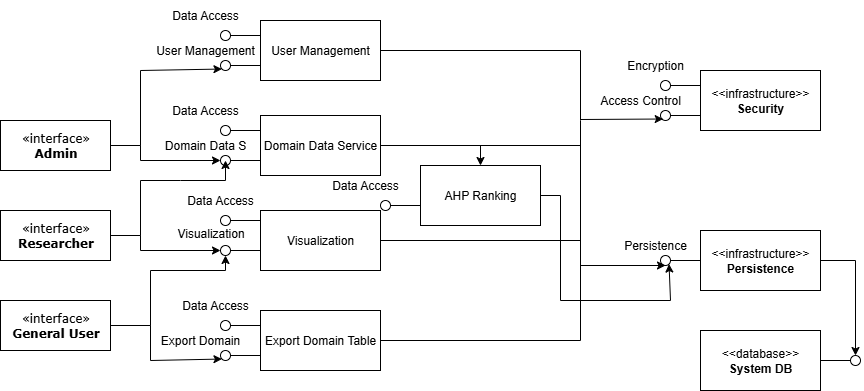
\includegraphics[scale=0.5] {component.png}
\end{figure}

\section{Critical Assumptions}

The following assumptions support hazard identification and mitigation:

\begin{itemize}
    \item \textbf{Access to Public APIs:} It is assumed that GitHub API and other
    data sources will remain stable; however, if access limits or outages occur,
    fallback mechanisms (e.g., cached data, manual upload) will be implemented.
    
    \item \textbf{McMaster Infrastructure Availability:} University servers will
    host the tool; if unavailable, contingency hosting (local or alternative
    cloud) will be explored.
    
    \item \textbf{Stable Development Team:} All members remain active; if a
    member becomes unavailable, roles and documentation ensure continuity.
    
    \item \textbf{Non-Safety-Critical Context:} Hazards relate to data and
    usability, not physical harm, but errors could still cause loss of
    credibility or project delays.
    
    \item \textbf{Defined Scope and Requirements:} Requirements remain stable;
    changes will trigger re-assessment of risks.
    
    \item \textbf{Version Control and Standards:} Git workflow reduces
    integration errors, though merge conflicts remain possible; peer reviews
    mitigate these.
    
    \item \textbf{User Feedback Availability:} Testing feedback will be
    accessible; if delayed, internal testing will substitute temporarily.
\end{itemize}

\section{Failure Mode and Effect Analysis}
The following contain our Failure Mode and Effect Analysis table is a breakdown of the hazards that could occur within the system, along with recommended actions to mitigate them.
\newgeometry{margin=0.5in}
\begin{landscape}
  \begin{longtable}{|p{3cm}|p{3cm}|p{4cm}|p{4cm}|p{3cm}|p{2cm}|p{3cm}|}
  \caption{Failure Mode and Effect Analysis} \label{FMEA}\\
  \hline
   Component & Failure Modes & Effects of Failure & Causes of Failure & Recommended Action & SR & Ref.  \\ 
  \hline
  \endfirsthead
  \multicolumn{7}{r}{Table \thetable\ Continued from previous page}\\ 
  \hline
   Design Function & Failure Modes & Effects of Failure & Causes of Failure & Recommended Action & SR & Ref.  \\ 
  \hline
  \endhead
  \multicolumn{7}{r}{{Continued on next page}}\\
  \endfoot
  \multicolumn{7}{r}{{Concluded}}\\
  \endlastfoot
  \multirow{7}{*}{User account} & 
  \begin{enumerate}[leftmargin=*]
    \item User can't log-in/sign-up.
    \item Cannot set correct role for user.
    \item User account information is leaked.
  \end{enumerate} & 
  \begin{enumerate}[leftmargin=*]
    \item User cannot access their work.
    \item Refer to H1-1.
    \item User credentials are exposed, exposing them to cyber attack or data scrapers.
  \end{enumerate} &
  \begin{enumerate}[leftmargin=*]
    \item
    \begin{enumerate}
        \item[a)] Integration with database failure.
        \item[b)] User entered incorrect credentials.
    \end{enumerate}
    \item Refer to H1-1.a.
    \item Weak access controls, lack of encryption, or insecure credentials.
  \end{enumerate} &
  \begin{enumerate}[leftmargin=*]
    \item 
    \begin{enumerate}
        \item[a)] Implement automated daily system integration testing.
        \item[b)] Provide user feedback during user actions.
    \end{enumerate}
    \item Refer to H1-1.a, H1-1.b.
    \item Implement Multi-factor authentication and follow industry best practices for security.
  \end{enumerate} &
  \begin{enumerate}[leftmargin=*]
    \item TODO
    \item TODO
    \item TODO
  \end{enumerate} &
  \begin{enumerate}[leftmargin=*]
    \item H1-1
    \item H1-2
    \item H1-3
  \end{enumerate} \\
  \hline
    Domain Creation & 
  \begin{enumerate}[leftmargin=*]
      \item Cannot create new domains
      \item Cannot edit existing domain
  \end{enumerate} & 
  \begin{enumerate}[leftmargin=*]
    \item
    \begin{enumerate}
        \item[a)] User cannot continue their work on the domain
        \item[b)] User will be delayed when writing their analysis
    \end{enumerate}
    \item Refer to H2-1.a, H2-1.b.
  \end{enumerate} &
  \begin{enumerate}[leftmargin=*]
    \item  Refer to H1-1.a
    \begin{enumerate}
        \item[a)] User has incorrect role credentials
    \end{enumerate}
    \item Refer to H1-1.a, H2-1.a.
  \end{enumerate} &
  \begin{enumerate}[leftmargin=*]
       \item Refer to H1-1.a, H1-1.b.
       \item  Refer to H1-1.a, H1-1.b.
  \end{enumerate} &
  \begin{enumerate}[leftmargin=*]
       \item TODO
       \item TODO
  \end{enumerate} &
  \begin{enumerate}[leftmargin=*]
       \item H2-1
       \item H2-2
  \end{enumerate} \\
  \hline
  Adding Data to Domain & 
  \begin{enumerate}[leftmargin=*]
      \item User cannot add new data point
      \item User cannot update existing data point
      \item Automated process overwriting user data unknowingly
      \item Automated data input failure
  \end{enumerate} & 
  \begin{enumerate}[leftmargin=*]
      \item Refer to H2-1.a, H2-1.b.
      \item Refer to H2-1.a, H2-1.b.
      \item Refer to H2-1.a, H2-1.b 
      \begin{enumerate}
        \item[a)] Loss of user trust towards the tool
    \end{enumerate}
      \item Refer to H2-1.a, H2-1.b,
      \begin{enumerate}
        \item[a)] User has to manually input data, reducing usefulness of the tool
    \end{enumerate}
  \end{enumerate} &
  \begin{enumerate}[leftmargin=*]
       \item Refer to H1-1.a
       \begin{enumerate}
            \item[a)] Network issues
            \item[b)] Save conflict occurring when multiple users are trying to edit the same data point
        \end{enumerate}
       \item Refer to H1-1.a, H3-1.a, H3-1.b
       \item 
       \begin{enumerate}
            \item[a)] Lack of user training on how automated data points work
            \item[b)] Inadequate user feedback user during system processes
        \end{enumerate}
       \item Refer to H3-1.a.
       \begin{enumerate}
            \item[a)] Integration issues with external systems
        \end{enumerate}
  \end{enumerate} &
  \begin{enumerate}[leftmargin=*]
    \item Refer to H1-1.a, H1-1.b.
    \begin{enumerate}
        \item[a)] Explicit visual block on data points that other users are editing
    \end{enumerate}
    \item Refer to H1-1.a, H1-1.b, H3-1.a.
    \item Refer to H1-1.a, H1-1.b
    \begin{enumerate}
        \item[a)] Provide explicit user controls for manual inputs
        \item[b)] Provide training on key features to user
        \item[c)] Implement confirmation system for automated sections
    \end{enumerate}
    \item Refer to H1-1.a, H1-1.b, H3-1.a.
  \end{enumerate} &
  \begin{enumerate}[leftmargin=*]
    \item TODO
    \item TODO
    \item TODO
    \item TODO

  \end{enumerate} &
  \begin{enumerate}[leftmargin=*]
    \item H3-1
    \item H3-2
    \item H3-3
    \item H3-4
  \end{enumerate} \\
  \hline
 Data Visualization & 
  \begin{enumerate}[leftmargin=*]
      \item Visualization method does not match data points
  \end{enumerate} & 
  \begin{enumerate}[leftmargin=*]
      \item Refer to H2-1.b, H3-3.a.
  \end{enumerate} &
  \begin{enumerate}[leftmargin=*]
    \item Refer to H1-1.a
    \begin{enumerate}
        \item[a)] External system used for visualization not properly configured/working
        \item[b)] Another user is editing the data points while current user is trying to visualize
    \end{enumerate}
  \end{enumerate} &
  \begin{enumerate}[leftmargin=*]
    \item Refer to H1-1.A
    \begin{enumerate}
        \item[a)] Require user to lock the domain when editing, with visualization functionality being available only on un-locked domains.
    \end{enumerate}
  \end{enumerate} &
  \begin{enumerate}[leftmargin=*]
       \item TODO
  \end{enumerate} &
  \begin{enumerate}[leftmargin=*]
       \item H4-1
  \end{enumerate} \\
  \hline
 Download Data  & 
  \begin{enumerate}[leftmargin=*]
    \item User unable to download the data/visuals of a domain
    \item Downloaded data/visuals of a domain are corrupted and unusable
  \end{enumerate} & 
  \begin{enumerate}[leftmargin=*]
      \item Refer to H2-1.b.
      \item Refer to H2-1.b, H3-3.a.
  \end{enumerate} &
  \begin{enumerate}[leftmargin=*]
    \item Refer to H1-1.a, H2.1.a, H3-1.a, H4-1.a.
    \item Refer to H1-1.a, H3-1.a, H4-1.a.
  \end{enumerate} &
  \begin{enumerate}[leftmargin=*]
       \item Refer tp H1-1.a, H1-1.b.
       \begin{enumerate}
        \item[a)] Provide multiple methods for downloading or sharing
    \end{enumerate}
       \item Refer tp H1-1.a, H1-1.b.
       \begin{enumerate}
        \item[a)] Implement proper error handling in code to catch exceptions
    \end{enumerate}
  \end{enumerate} &
  \begin{enumerate}[leftmargin=*]
       \item TODO
       \item TODO
  \end{enumerate} &
  \begin{enumerate}[leftmargin=*]
       \item H5-1
       \item H5-2
  \end{enumerate} \\
  \hline
  \end{longtable}
\end{landscape}
\restoregeometry


\section{Safety and Security Requirements}
The hazard analysis revealed several safety-related requirements that were not fully covered in the SRS.
These requirements aim to prevent data loss, improve user experience during failures, and keep the tool reliable.

\subsection*{Clear Error Feedback and Account Recovery}
The system must show clear error messages (e.g., wrong password, network failure) and give users a way to reset their credentials if they forget them.

\subsection*{Correct Role Assignment}
User roles (Viewer / Contributor) must be assigned and saved correctly at sign-up or when updated by an admin so that permissions are always accurate.

\subsection*{Protecting Manual Edits from Automated Updates}
If automated data refreshes could overwrite a user’s manual entry, the system must warn the user or ask for confirmation before replacing the data.

\subsection*{Preventing Conflicting Edits}
When two people try to edit the same record at the same time, the tool must either block one of the saves or clearly warn the users to avoid losing data.

\subsection*{Consistent Visualization}
Publishing visualizations must not happen at the same time as ongoing data edits.
The system should either block publishing during edits or enforce a short downtime so charts and scores always reflect a stable dataset.

\subsection*{Reliable Download of Data and Visuals}
If an export (CSV, PNG, etc.) fails or the file is corrupted, the tool must alert the user and, where possible, let them retry the download.

\section{Roadmap}

For the Capstone timeline, we will focus on the safety features that are needed to make the tool work properly:

\begin{itemize}
    \item Login with account recovery so that users can sign in securely.
    \item Correct role assignment (Viewer / Contributor) so only authorized users can edit data.
    \item A basic warning when automated updates might overwrite manual edits.
    \item Reliable downloads for tables and charts, with a simple error message if something goes wrong.
\end{itemize}

Some features will be added later as future improvements:

\begin{itemize}
    \item A better system to prevent publishing visualizations while edits are happening (for example, temporary downtime or blocking the publish button).
    \item A stronger solution for conflicting edits, such as proper locking or live conflict warnings.
    \item More advanced error handling for things like failed downloads or export retries.
\end{itemize}


\newpage{}

\section*{Appendix --- Reflection}

\wss{Not required for CAS 741}

The purpose of reflection questions is to give you a chance to assess your own
learning and that of your group as a whole, and to find ways to improve in the
future. Reflection is an important part of the learning process.  Reflection is
also an essential component of a successful software development process.  

Reflections are most interesting and useful when they're honest, even if the
stories they tell are imperfect. You will be marked based on your depth of
thought and analysis, and not based on the content of the reflections
themselves. Thus, for full marks we encourage you to answer openly and honestly
and to avoid simply writing ``what you think the evaluator wants to hear.''

Please answer the following questions.  Some questions can be answered on the
team level, but where appropriate, each team member should write their own
response:


\begin{enumerate}
    \item What went well while writing this deliverable?
    \\\textbf{Haniye:} One thing that went well was that looking at the hazards helped us spot requirements we hadn’t considered before. Thinking through the risks made certain scenarios much clearer, like what happens if login fails or downloaded file is corrupted.
    \item What pain points did you experience during this deliverable, and how
    did you resolve them?
    \\\textbf{Haniye:} One challenge was figuring out which safety features to prioritize for the Capstone demo and which to leave for later. After looking at the project scope, we agreed to focus on the most essential features that would keep the tool stable and reliable for the demo.
    \item Which of your listed risks had your team thought of before this
    deliverable, and which did you think of while doing this deliverable? For
    the latter ones (ones you thought of while doing the Hazard Analysis), how
    did they come about?
    \\\textbf{Haniye:} Some hazards were already on our radar but only partially covered in the original requirements. For example, we had noted the risk of conflicting edits and planned to keep a record of changes, but we hadn’t considered that the system should also block or warn other users editing the same record. Similarly, we knew we’d have different user roles, but we overlooked the need to handle role assignment correctly in the database. Other risks, like login failures or charts showing incomplete data, only came up as we worked through the hazard analysis and FMEA table.
    \item Other than the risk of physical harm (some projects may not have any
    appreciable risks of this form), list at least 2 other types of risk in
    software products. Why are they important to consider?
    \\\textbf{Haniye:} N/A
\end{enumerate}

\end{document}